
\section{Phân tích bổ sung kết quả thực nghiệm}

\subsection{Số frequent itemset theo minsup và mật độ dữ liệu}

Hình~\ref{fig:pattern-counts} so sánh số mẫu của backend bitset ở sáu
ngưỡng. MinSup được biểu diễn theo tỷ lệ của support singleton lớn nhất
riêng từng bộ dữ liệu; do đó đây không phải cùng một ngưỡng support tuyệt
đối giữa các bộ. Trục tung dùng thang logarit cơ số 2 để thể hiện đồng thời
các tập dữ liệu có kích thước đầu ra khác nhau.

\begin{figure*}[!t]
\centering
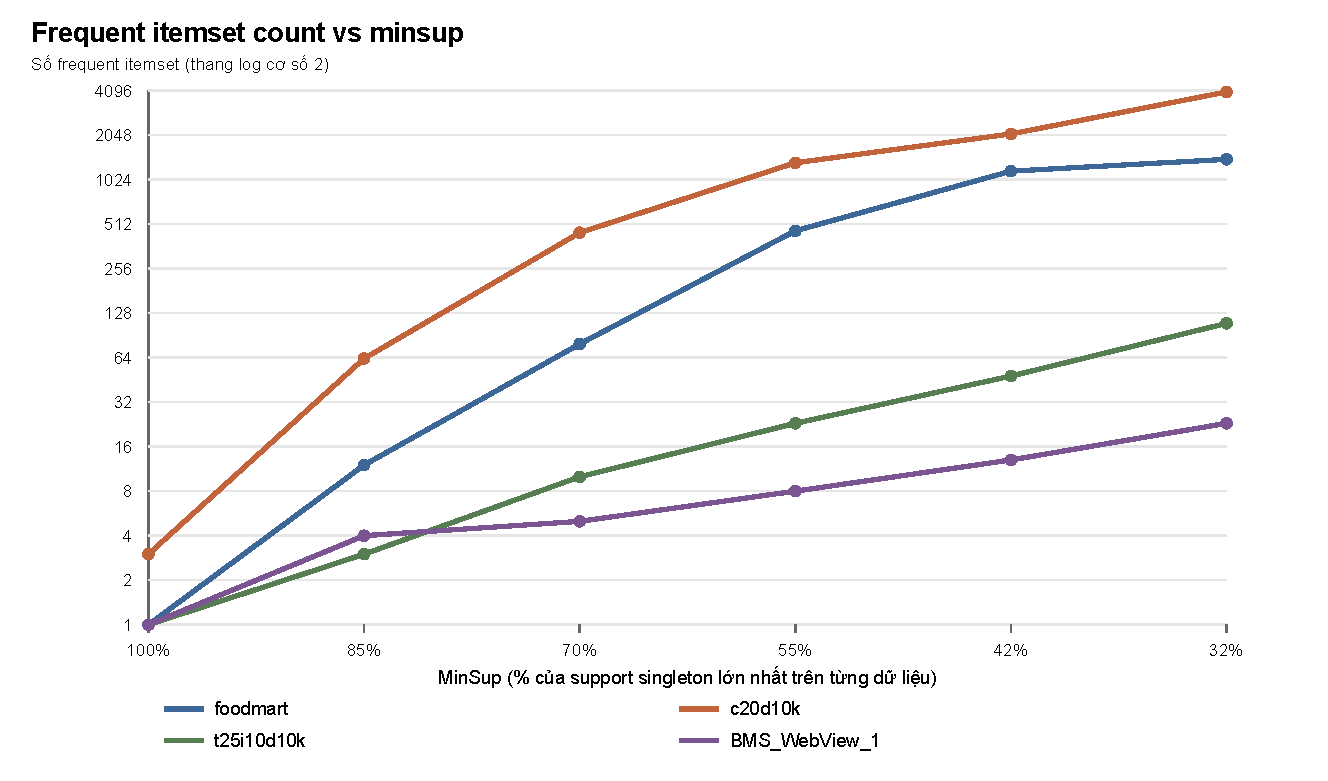
\includegraphics[width=0.82\textwidth]{figures/patterns.pdf}
\caption{Số frequent itemset theo minsup trên bốn bộ benchmark.}
\label{fig:pattern-counts}
\end{figure*}

Khi minsup giảm từ mức cao nhất xuống thấp nhất, số itemset tăng trên cả
bốn bộ: c20d10k từ 3 lên 3999, Foodmart từ 1 lên 1400, t25i10d10k từ 1
lên 109 và BMS\_WebView\_1 từ 1 lên 23. Theo thống kê parser, mật độ giao
dịch ước lượng bằng độ dài giao dịch trung bình chia số item phân biệt lần
lượt xấp xỉ 10.42\% với c20d10k, 2.67\% với t25i10d10k, 0.51\% với
BMS\_WebView\_1 và 0.28\% với Foodmart. Kết quả phù hợp với xu hướng dữ
liệu dày hơn tạo nhiều tổ hợp phổ biến hơn trong các cấu hình đã thử; tuy
nhiên đây không phải quan hệ nhân quả được cô lập, vì số giao dịch, phân
bố item và các ngưỡng support tuyệt đối khác nhau giữa các bộ.

\subsection{Ảnh hưởng của ngưỡng support}

Trên Foodmart, khi ngưỡng support tuyệt đối giảm từ
25 xuống 8, số frequent itemset tăng từ 1 lên 1400.
Thời gian của backend set tăng từ 0.026090 lên
1.021860 giây. Backend bitset tăng từ 0.024859
lên 0.892147 giây. Kết quả cho thấy chi phí khai
thác chịu ảnh hưởng đáng kể bởi số lượng itemset
được tìm thấy, không chỉ bởi kích thước dữ liệu.

\begin{figure*}[!t]
\centering
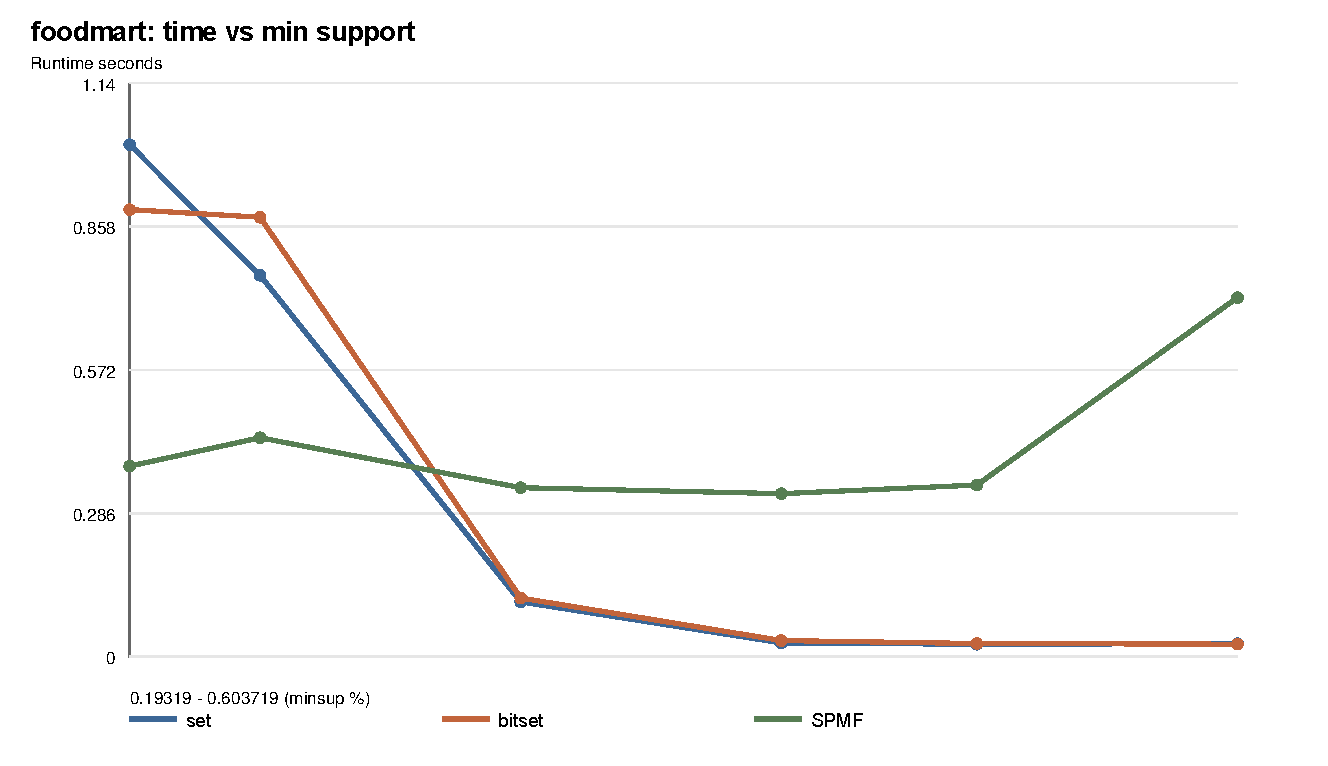
\includegraphics[width=0.85\textwidth]{figures/foodmart.pdf}
\caption{Thời gian chạy Eclat trên Foodmart theo ngưỡng support.}
\label{fig:foodmartreal}
\end{figure*}

\subsection{So sánh TID-set và bitset}

Ở c20d10k với ngưỡng support tuyệt đối 3200,
backend set mất 0.685201 giây, trong khi bitset
mất 0.303265 giây. Như vậy, bitset nhanh khoảng
2.26 lần trong cấu hình này. Tuy nhiên, sự khác
biệt không đồng nhất ở tất cả các ngưỡng,
nên không thể kết luận bitset luôn nhanh hơn.

\begin{figure*}[!t]
\centering
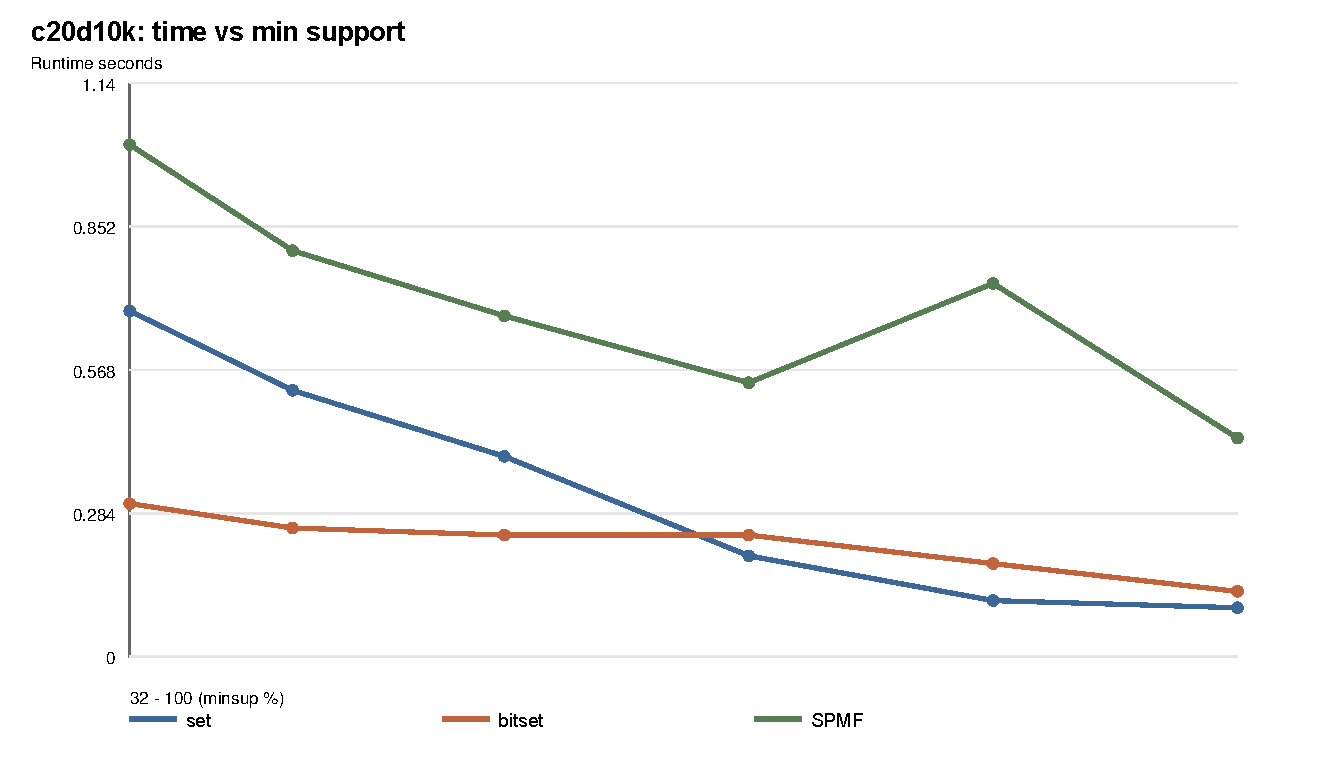
\includegraphics[width=0.85\textwidth]{figures/c20.pdf}
\caption{So sánh thời gian của hai backend trên c20d10k.}
\label{fig:c20real}
\end{figure*}

\subsection{Đặc điểm dữ liệu web thưa}

BMS\_WebView\_1 có 59602 giao dịch và 497 item
khác nhau. Khi minsup giảm từ 3658 xuống 1171
giao dịch, số frequent itemset tăng từ 1 lên 23.
Trong các phép đo đã thực hiện, backend set có
thời gian thấp hơn bitset ở một số ngưỡng,
cho thấy hiệu quả của biểu diễn dữ liệu còn phụ
thuộc vào phân bố giao dịch.

\begin{figure*}[!t]
\centering
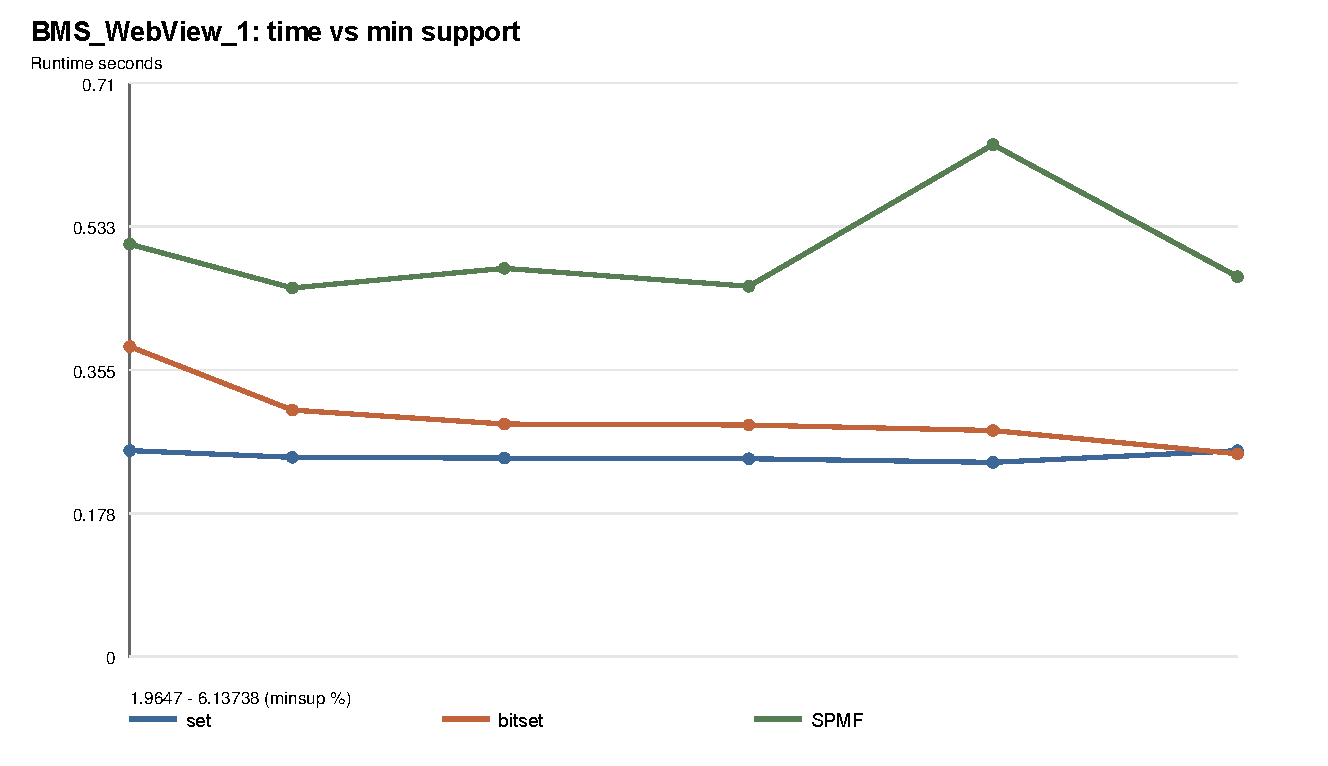
\includegraphics[width=0.85\textwidth]{figures/bms.pdf}
\caption{Thời gian chạy Eclat trên BMS WebView 1.}
\label{fig:bmsreal}
\end{figure*}

\subsection{Đánh giá bộ nhớ}

Biểu đồ bộ nhớ Python của c20d10k đo bằng
tracemalloc, chỉ phản ánh các cấp phát được Python
theo dõi. Phép đo RSS trong tiến trình riêng tại
minsup 5500 ghi nhận 85.2305 MiB với backend set
và 62.8398 MiB với backend bitset. Hai loại phép
đo không được xem là tương đương.

\begin{figure*}[!t]
\centering
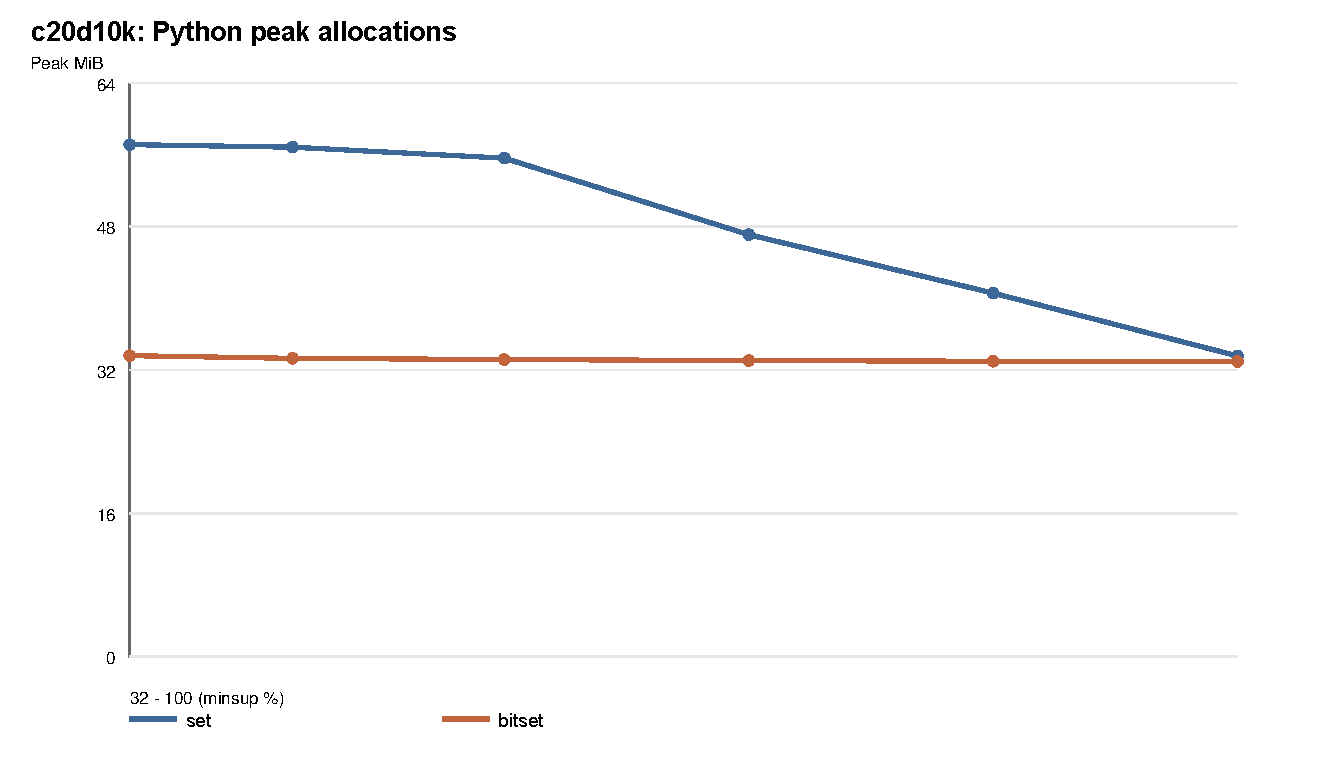
\includegraphics[width=0.85\textwidth]{figures/memory.pdf}
\caption{Bộ nhớ cấp phát Python trên c20d10k, đo bằng tracemalloc.}
\label{fig:memoryreal}
\end{figure*}

\subsection{Khả năng mở rộng}

Thí nghiệm scalability sử dụng lần lượt
10\%, 25\%, 50\%, 75\% và 100\% số giao dịch
của BMS\_WebView\_1. Khi tăng từ 5960 lên
59602 giao dịch, thời gian chạy tăng từ
0.043374 lên 0.472338 giây. Các kết quả
cho thấy xu hướng tăng thời gian theo quy mô
dữ liệu trong cấu hình đã đo, nhưng chưa đủ
để khẳng định một độ phức tạp tiệm cận cụ thể.

\begin{figure*}[!t]
\centering
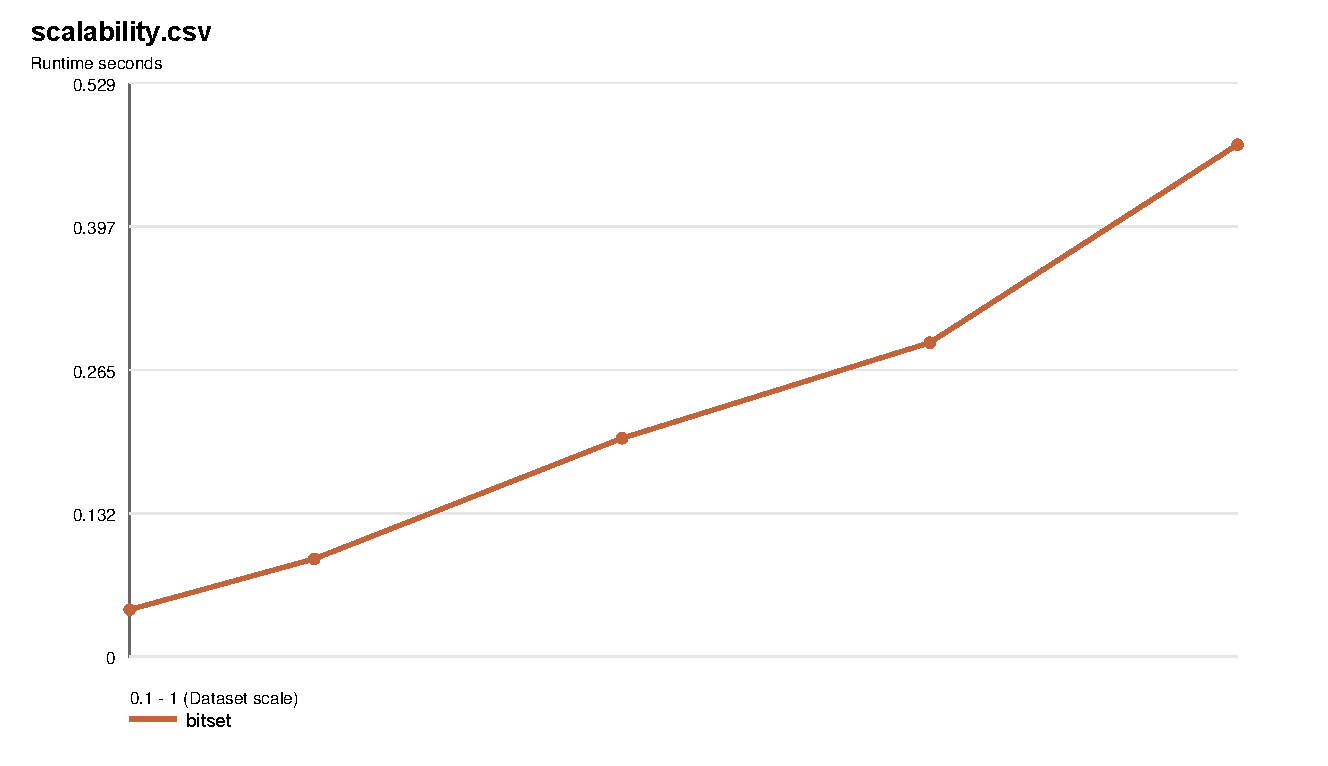
\includegraphics[width=0.85\textwidth]{figures/scalability.pdf}
\caption{Khả năng mở rộng của backend bitset trên BMS WebView 1.}
\label{fig:scalabilityreal}
\end{figure*}

\subsection{Ảnh hưởng của độ dài giao dịch}

Khi độ dài giao dịch trung bình thay đổi từ
3 đến 11 trong bộ dữ liệu tổng hợp, thời gian
chạy ghi nhận lần lượt là 0.009214 và
0.019488 giây ở hai đầu khoảng thử nghiệm.
Số frequent itemset tương ứng tăng từ 52
lên 285. Sự biến thiên này cho thấy độ dài
giao dịch có thể ảnh hưởng đến số tổ hợp
cần xử lý; đồng thời sự thay đổi phân bố
item trong dữ liệu tổng hợp cũng phải được
xem xét khi diễn giải.

\begin{figure*}[!t]
\centering
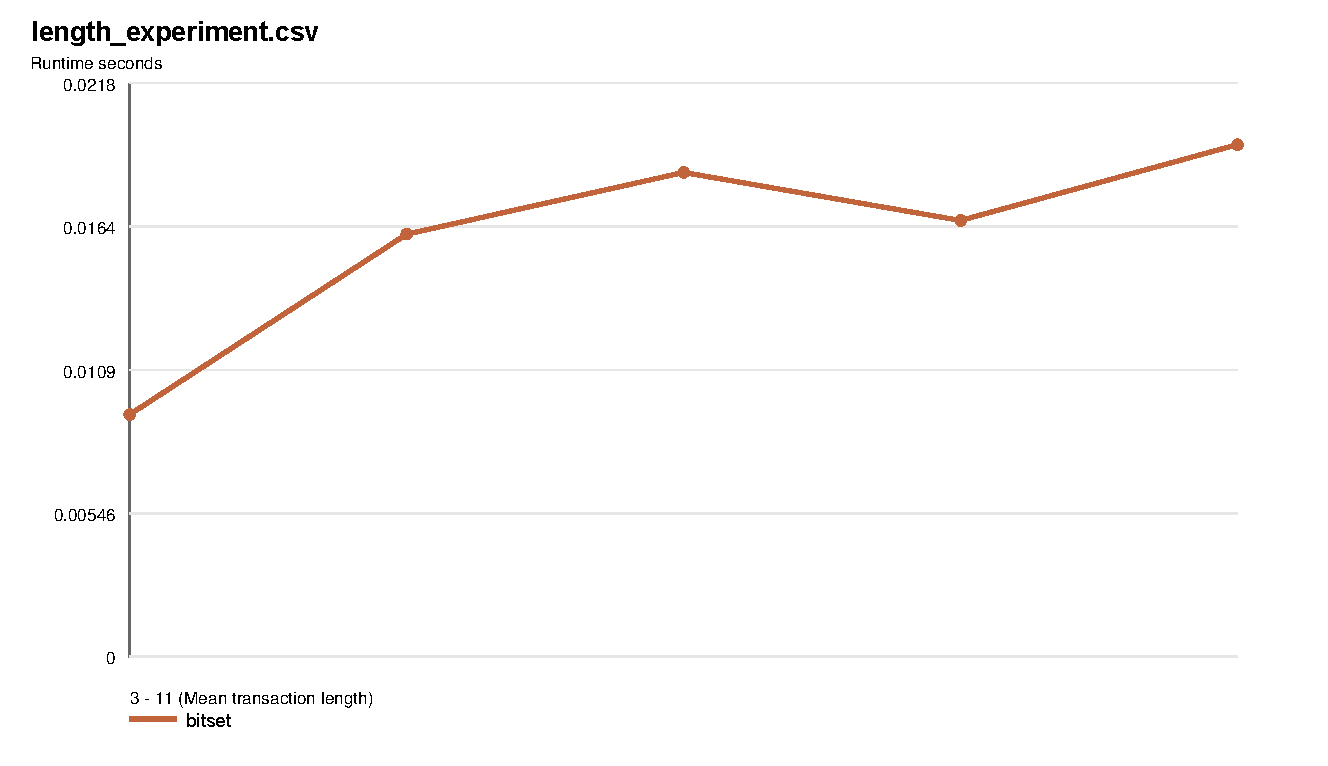
\includegraphics[width=0.85\textwidth]{figures/length.pdf}
\caption{Thời gian chạy theo độ dài giao dịch trong dữ liệu tổng hợp.}
\label{fig:lengthreal}
\end{figure*}

\subsection{Giới hạn của kết quả}

Các thời gian trên là phép đo thực nghiệm
trên môi trường đã sử dụng và chưa được
đại diện bằng trung bình từ nhiều lần chạy.
Thời gian khởi động JVM trong phép chạy SPMF
không thể so sánh trực tiếp với thời gian
khai thác trong tiến trình Python.
Những giới hạn này cần được tính đến khi
đánh giá hiệu năng của Eclat.
